\noindent Algebraic reasoning aims to abstract the IK-Sphere problem and formally generalise it to the unfamiliar four and above dimensions.

\section{The Radius of the IK-Sphere as Dimension Tends to Infinity}
The radius $r$ of the IK-Sphere can be solved for algebraically and generalised by extending the Pythagorean Theorem.
\begin{lemma}[Extended Pythagorean Theorem for $n$-cube]\label{lemma:extend pythag}
    For an $n$-cube in $n$-dimensions, with a set of lines of length $a_1, a_2, a_3, ... , a_n$, each perpendicular to all others and originating from the same vertex, the length of the diagonal $c$ of the $n$-cube is given by
    \begin{equation}\label{extendedpythag}
        c^2 = \sum_{i}^{n}a_i^2
    \end{equation}
\end{lemma}
\begin{proof}

    Assuming the original two-dimensional Pythagorean Theorem is proven,
    
    \noindent 
    Base case $\left(n=3\right)$
    \begin{equation*}
        \begin{split}
            c^2&=1^2+1^2+1^2\\
            c&=\sqrt{3}
        \end{split}
    \end{equation*}
    So, the lemma holds for $n=3$.
    
    \noindent Inductive hypothesis: Suppose the theorem holds for all values of $n$ up to some $k$, $k \geq 3$.
    \begin{equation*}
        \begin{split}
            c^2=\sum_{i}^{k}a_i^2
        \end{split}
    \end{equation*}
    
    \noindent Inductive step: Let $n=k+1$. 
    \begin{equation*}
        \begin{split}
        \sum_{i}^{k+1}a^2_{i}
        \end{split}
    \end{equation*}
    Then our right side is
    \begin{equation*}
        \begin{split}
        \sum_{i}^{k}a_i^2+a_{i+1}^2=\sum_{i}^{k+1}a^2_{i}
        \end{split}
    \end{equation*}
    which is our left side. So, the theorem holds for $n=k+1$. 
    By the principle of mathematical induction, the theorem holds for all $n \in \mathbb{N}$.
\end{proof}
Let us use a diagram for a 2D IK-Sphere to generalise the IK-Sphere radius $r_n$ to $n$-dimensions. Using the Extended Pythagorean Theorem for an $n$-cube we can determine the length of a diagonal (see line $\overline{\rm AB}$ in Figure \ref{fig:2d diagonal}) of a quadrant of our 2-cube that includes a unit $n$-sphere radius and the radius of the IK-Sphere which we wish to obtain. 
\begin{figure}[h]
    \centering
    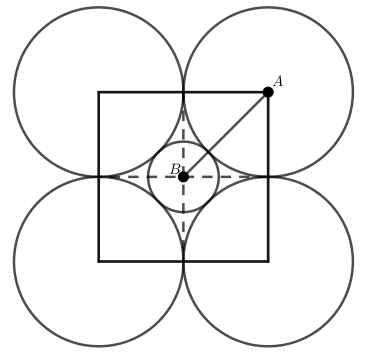
\includegraphics[width=0.4\textwidth]{images/diagonal 2d.png}
    \caption{\label{fig:2d diagonal}Unit 2-cube diagonal length determined using Extended Pythagorean Theorem}
\end{figure}

\noindent Hence, we can subtract the unit circle radius to obtain the radius of the two-dimensional IK-Sphere: $$r_2 = \sqrt{1^2+1^2}-1.$$  %Then, dividing by 2, we get the radius of an IK-Sphere in two-dimensions: $$r_2=\frac{\sqrt{1^2+1^2}-2}{2}.$$ 

Similarly, for a three-dimensional IK-Sphere, the length of the diagonal is the square root of the sum of three sides of of an octant of the $n$-cube at a vertex (see Figure \ref{fig:3d diagonal}). From there, the process is the same and we subtract the unit sphere. Thus, we have an inscribed sphere radius $r_3$ of: 

\begin{equation*}
    r_3=\sqrt{1^2+1^2+1^2}-1.
\end{equation*}

\begin{figure}[H]
    \centering
    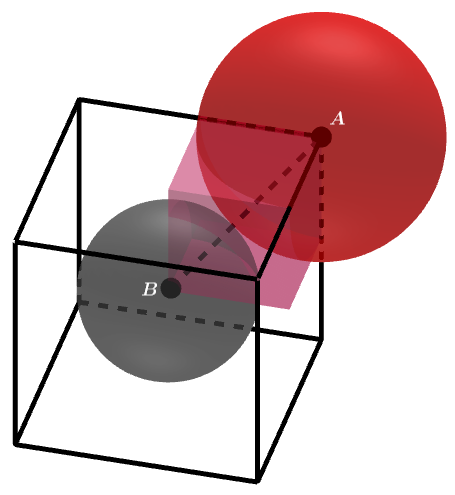
\includegraphics[width=0.6\textwidth]{images/3d diagonal.png}
    \caption{\label{fig:3d diagonal}Unit 3-cube diagonal length determined using Extended Pythagorean Theorem}
\end{figure}

\begin{corollary}[To the Extended Pythagorean Theorem for $n$-Cubes] The diagonal $c$ of a unit $n$-cube is given by
\begin{equation} \label{ncube diagonal}
    c = \sqrt{n}
\end{equation}
\end{corollary}
\begin{proof}
    Substituting $a=1$ into the extended Pythagorean Theorem (see Equation \ref{extendedpythag}), we have
    \begin{align*}
        c^2 &= \sum_{i}^{n}1_i^2\\
        &=n\\
        \therefore c &= \sqrt{n}.
    \end{align*}
\end{proof}

If the diagonal of a unit $n$-cube is given by $\sqrt{n}$ (see Equation \ref{ncube diagonal}), the IK-Sphere radius can be generalised across all $n$-dimensions by subtracting the unit sphere radius as follows:
\begin{equation}\label{radius of ik sphere}
    r_n = \sqrt{n}-1
\end{equation}

We may now proceed to the final step of proving that the radius of an IK-Sphere increases without bound.

\begin{theorem}
As the dimension $n$ tends to infinity, the radius $r_n$ of the inscribed sphere also tends to infinity.
\end{theorem}
\begin{proof}
Take the limit as $n$ approaches infinity of the expression for $r_n$ in terms of $n$ (See Equation \ref{radius of ik sphere}) and apply the difference law:
\begin{align*}
    \lim_{n\to\infty} \sqrt{n}-1 &= \lim_{n\to\infty} \sqrt{n} - \lim_{n\to\infty} \sqrt{1}\\
    &=\infty - 1\\
    &=\infty
\end{align*}
$\therefore$ the radius of an IK-Sphere diverges to infinity as dimension $n$ increases.\\
\end{proof}

Graphically (see Figure \ref{fig:radius increases graph}), we may observe the same result with less rigour. The domain has been restricted to $n\geq3$ as $n=3$ was the base case for the Extended Pythagorean Theorem for an $n$-Cube (see Lemma \ref{lemma:extend pythag}). Below $n=1$ we obtain negative values for $r_n$ which can accordingly be considered undefined region. Investigation into fractional dimensions could reveal a reason, however, that is currently beyond the scope of this essay.
%Here begins the 2D plot
\begin{figure}[H]
    \centering
    \begin{tikzpicture}
        \begin{axis}[
            axis lines = left,
            xlabel = \(n\),
            ylabel = {\(r_n\)},
        ]
        %Below the red parabola is defined
        \addplot [
            domain=3:100, 
            samples=100, 
            color=red,
        ]
        {sqrt(x)-1};
        \addlegendentry{\(\sqrt{n}-1\)}
        %Here the blue parabola is defined
        \end{axis}
    \end{tikzpicture}
    \caption{Caption}
    \label{fig:radius increases graph}
\end{figure}
%Here ends the 2D plot






\section{Verification of the IK-Sphere at Nine Dimensions}
The radius of an IK-Sphere has now been proven to increase without bound. As such, one may infer that the IK-Sphere bursts outside of its bounding box as dimensionality increases, implying that there exist intersection points between the IK-Sphere and its `bounding' $n$-cube at higher dimensions. In fact, upon inspection, one may observe that at $n=4$ dimensions, $$r_4=\sqrt{4}-1=1.$$ The IK-Sphere fits perfectly within its bounding 4-cube with side length 2 units (!). Here, intuition takes hold once again. One may assume there exists a solvable intersection point on a single face of the 4-cube with the IK-Sphere. However, another possibility arises in which higher dimensional intersections may operate differently and the IK-Sphere may still exist within its bounding $n$-cube as we originally assumed. We can verify the existence, or lack thereof, of an intersection point to decide which of these possibilities is true in higher dimensions.

From the definition of an $n$-sphere (see Definition \ref{def:n-sphere}) the following equation can be constructed:
\begin{equation}\label{eq:unit 4-sphere}
    x_1^2+y_2^2+z_3^2+w_4^2=1
\end{equation}
where $(x, y, z, w)$ is a point on the 4-sphere.

However, this does not help our high dimensional intuition. As such, geometric reasoning is required.

